\ifdefined \buildingFullOPALManual \else


%\ifx \@buildingFullOPALManual \@empty
%\else

%\documentclass[12pt,a4paper]{report}
\documentclass[a4paper]{book}

%% does not work in Latex2Html mode
%\usepackage{hyperref}

\usepackage[T1]{fontenc}
\usepackage{url}
\usepackage{html}
\usepackage{epic}
\usepackage{eepic}
\usepackage{makeidx}
\usepackage{array}
\usepackage{times}
\usepackage{amsmath}
\usepackage{amsxtra}
\usepackage{bm}
\usepackage[thin,thinp,thinc]{esdiff}
\usepackage{etoolbox}
\usepackage{graphicx}
\usepackage{dingbat}
\usepackage{color}
\usepackage{subfig}
\usepackage{boxedminipage}
\usepackage{alltt}
\usepackage{nicefrac}
\usepackage{calc}
%\usepackage{pdfdraftcopy}             % Draft
\usepackage{tikz}
\usetikzlibrary{
  er,3d,calc,fadings,trees,positioning,arrows,chains,decorations.pathreplacing,
  decorations.pathmorphing,shapes,shapes.symbols,shapes.arrows,matrix,through,decorations.text
}

\tikzset{
  >=stealth',
  punktchain/.style={rectangle,rounded corners, draw=black, very thick,text width=10em,
                     minimum height=3em, text centered, on chain},
  line/.style={draw, thick, <-},
  element/.style={tape,top color=white,bottom color=blue!50!black!60!,minimum width=8em,
                  draw=blue!40!black!90, very thick,text width=10em, minimum height=3.5em,
                  text centered, on chain},
  every join/.style={->, thick,shorten >=1pt},
  tuborg/.style={decorate},
  tubnode/.style={midway, right=2pt}
}

\tikzstyle{material}=[draw, fill=blue!20, text width=16.0em, text centered, minimum height=1.5em]
\tikzstyle{diagramstep} = [material, text width=20em, minimum width=10em, minimum height=3em, rounded corners]
\tikzstyle{line} = [draw, thick, color=black!50, -latex']

\usepackage{booktabs}
\usepackage{xspace}
\usepackage{xstring}

\usepackage{fancyvrb}
\usepackage{rotating}
\usepackage{float}

\usepackage{tabularx}
\usepackage{longtable}
\setcounter{LTchunksize}{3}

\usepackage[section]{placeins}
\usepackage{MnSymbol}
\usepackage{microtype}
\usepackage{setspace}
\usepackage{dcolumn}

\usepackage[vmargin={3.0cm,3.0cm},
            hmargin={2.0cm,3.0cm}]{geometry}

\usepackage{upgreek}
\usepackage[binary-units=true]{siunitx}
\sisetup{exponent-product = \cdot,math-ohm=\Upomega,text-ohm=\ensuremath{\Upomega}}
\DeclareSIUnit{\clight}{c}
\DeclareSIUnit\gauss{Ga}

\usepackage{engord}
\usepackage{wasysym}
\DeclareSIUnit[number-unit-product = \,]{\permill}{\permil}

\usepackage{hyperref}
\hypersetup{
    pdftitle          = The OPAL Framework,
    pdfauthor         = {Andreas Adelmann, Achim Gsell, Valeria Rizzoglio, Christof Metzger-Kraus,
                         Yves Ineichen, Xiaoying Pang, Steve Russell, Chuan Wang, Jianjun Yang,
                         Suzanne Sheehy, Chris Rogers, Daniel Winklehner},
    pdfsubject        = User's Reference Manual,
    pdffitwindow      = true,               % page fit to window when opened
    pdfnewwindow      = true,               % links in new window
    colorlinks        = true,               % false: boxed links; true: colored links
    linkcolor         = black!80!green,     % color of internal links
    citecolor         = black!20!red,       % color of links to bibliography
    urlcolor          = blue,               % color of external links
    breaklinks        = true,
    bookmarksnumbered = true,
    plainpages        = false
}

\usepackage{ifthen}

\newif \iflinuxwindows
\linuxwindowstrue   % set this to true when building the manual on Linux or Windows
\iflinuxwindows
\usepackage{epstopdf}
\fi

\usepackage[backend=biber,
            style=phys,
            biblabel=brackets,
            maxnames=3,
            doi=true,
            isbn=true,
            url=true]{biblatex}
%---- macros ----

\renewcommand{\topfraction}{1.0}
\renewcommand{\bottomfraction}{1.0}
\renewcommand{\textfraction}{0.0}
\renewcommand{\arraystretch}{2.0}
\newenvironment{tex2html_nowrap}{}{}


\newcommand{\Newline}{\hfil \\}


\newsavebox{\ExampleBox}
\newenvironment{example}
 {\VerbatimEnvironment
  \begin{flushleft}
  \begin{lrbox}{\ExampleBox}
    \begin{minipage}{\linewidth}
  \begin{Verbatim}[frame=lines,xleftmargin=0cm,fontsize=\footnotesize,samepage=true]}
 {\end{Verbatim}
  \end{minipage}
  \end{lrbox}
  \mbox{\usebox{\ExampleBox}}
  \end{flushleft}
 }

\newenvironment{longexample}
{\Verbatim[frame=lines,xleftmargin=0mm,fontsize=\footnotesize]}
{\endVerbatim}

%\examplefromfile{filename} reads in a text file and displays it in the document.
\newcommand{\examplefromfile}[1]{
\VerbatimInput[frame=lines,xleftmargin=0mm,fontsize=\footnotesize,label=\texttt{#1}]{#1}}

%for upright d of differentials
\makeatletter
\newcount\my@repeat@count

\newcommand{\myrepeat}[2]{%
  \begingroup
  \my@repeat@count=\z@
  \@whilenum\my@repeat@count<#1\do{#2\advance\my@repeat@count\@ne}%
  \endgroup
}

\newcommand{\differential}[1]{\ifstrempty{#1}{\ES@dop\ES@difint}{\ES@dop^{#1}\ES@difint}}
\newcommand{\pdifferential}[1]{\ifstrempty{#1}{{\partial\,}}{{\partial^{#1}\,}}}

\makeatother

\newcommand{\der}[3][]{\frac{\differential{#1}#2}{\differential{}\ifstrempty{#1}{#3}{#3^#1}}}
\newcommand{\parder}[3][]{\frac{\pdifferential{#1}#2}{\pdifferential{}\ifstrempty{#1}{#3}{#3^#1}}}
\newcommand{\niceder}[3][]{\nicefrac{\differential{#1}#2}{\differential{}\ifstrempty{#1}{#3}{#3^#1}}}
\newcommand{\uglyder}[3][]{{\differential{#1}#2}/{\differential{}\ifstrempty{#1}{#3}{#3^#1}}}
\newcommand{\uglyparder}[3][]{{\pdifferential{#1}#2}/{\pdifferential{}\ifstrempty{#1}{#3}{#3^#1}}}
\newcommand{\dd}[1][]{\; \differential{#1}}
\newcommand{\primed}{^{\prime}}
\newcommand{\dprimed}{^{\prime\prime}}
\newcommand{\nprimed}[1]{^{\myrepeat{#1}{\prime}}}

%Editing Macros
\newcommand{\TODO}[1]{{\color{red}\ifthenelse{\boolean{ShowDebug}}{[TODO: #1]}{}}}



%text in gray box
\newsavebox{\fmbox}
\definecolor{lightgray}{gray}{0.95}
\newenvironment{fmpage}
   {\vspace{-1.0cm}\begin{lrbox}{\fmbox}\begin{minipage}[t]{13.5cm}\vspace{0.1cm}}
   {\vspace{-0.4cm}\end{minipage}\end{lrbox}\begin{center}\fcolorbox{black}{lightgray}{\usebox{\fmbox}}\end{center}}


% Definition new signes
\newcommand{\R}{{\mathbb R}} % real numbers
\newcommand{\Q}{{\mathbb Q}} % rational numbers
\newcommand{\Z}{{\mathbb Z}} % integer numbers
\newcommand{\N}{{\mathbb N}} % natural numbers

\newcommand{\mad}{\textsc{mad}\xspace}
\newcommand{\madnine}{\textsc{mad9}\xspace}
\newcommand{\madninep}{\textsc{mad9p}\xspace}
\newcommand{\madeight}{\textsc{mad8}\xspace}
\newcommand{\classic}{\textsc{classic}\xspace}

\makeatletter
\newcommand{\opal@impl}{\textsc{Opal}}
\newcommand{\opalt@impl}{\textsc{Opal-t}}
\newcommand{\opalcycl@impl}{\textsc{Opal-cycl}}
\newcommand{\opalmap@impl}{\textsc{Opal-map}}
\newcommand{\opalenv@impl}{\textsc{Opal-e}}

\newcommand{\opal}{\opal@impl\xspace}
\newcommand{\opalt}{\opalt@impl\xspace}
\newcommand{\opalcycl}{\opalcycl@impl\xspace}
\newcommand{\opalmap}{\opalmap@impl\xspace}
\newcommand{\opalenv}{\opalenv@impl\xspace}

\newcommand{\noopalt}{\leftthumbsdown \opalt@impl\xspace}
\newcommand{\noopalcycl}{\leftthumbsdown \opalcycl@impl\xspace}
\newcommand{\noopalmap}{\leftthumbsdown \opalmap@impl\xspace}
\newcommand{\noopalenv}{\leftthumbsdown \opalenv@impl\xspace}
\makeatother

\newcommand{\impactt}{\textsc{Impact-t}\xspace}
\newcommand{\partroot}{\textsc{H5root}}


\newcommand{\latermore}{More details will be given in Version 1.6.0}


\newcommand{\lieop}[1]{{:}{#1}{:}}

\newcommand{\rms}[1]{\overset{\sim}{#1}}

\newcommand{\sprod}{\cdot}
\newcommand{\vprod}{\times}
\newcommand{\matr}[1]{\mathcal{#1}}
\renewcommand{\vec}[1]{{\bm{#1}}}
\newcommand{\transpose}[1]{#1^\intercal}
\renewcommand{\epsilon}{\varepsilon}

\newcommand{\keyword}[2][]{\ifstrempty{#1}{\texttt{\expandafter\MakeUppercase\expandafter{#2}}}{\hyperref[#1]{\texttt{\expandafter\MakeUppercase\expandafter{#2}}}}}
\newcommand{\tabline}[3][]{\keyword[#1]{#2}& #3 \\}
\newcommand{\tabheadcell}[1]{{\bfseries #1}}

\newcommand*\kdescriptionlabel[1]{\hspace\labelsep
                                \normalfont\keyword{#1}\index{#1}}
\makeatletter
\newenvironment{kdescription}
               {\list{}{\labelwidth\z@ \itemindent-\leftmargin
                        \let\makelabel\kdescriptionlabel}}
               {\endlist}
\makeatother

\ExplSyntaxOn
\NewDocumentCommand{\tabhead}{ m }
 {
  \seq_set_split:Nnn \l_tmpa_seq { & } { #1 }
  \bfseries \seq_use:Nn \l_tmpa_seq { & \bfseries } \\
 }

\NewDocumentCommand \multrefImpl { O{ } m m m } {
  \ifnumgreater{\clist_count:n {#4}}{1}{
    \seq_set_from_clist:Nn \l_tmpa_seq { #4 }

    \seq_set_map:NNn \l_tmpb_seq \l_tmpa_seq { \exp_not:n { \ref{#3:##1} } }
    \ifstrempty{#1}{#2s}{#1}~\seq_use:Nnnn \l_tmpb_seq {\ and\ } {,\ } {,\ and\ }
  }{
    #2~\ref{#3:#4}
  }
}

\NewDocumentCommand \multeqnrefImpl { m } {
  \ifnumgreater{\clist_count:n {#1}}{1}{
    \seq_set_from_clist:Nn \l_tmpa_seq { #1 }

    \seq_set_map:NNn \l_tmpb_seq \l_tmpa_seq { \exp_not:n { \eqref{eq:##1} } }
    Equations~\seq_use:Nnnn \l_tmpb_seq {\ and\ } {,\ } {,\ and\ }
  }{
    Equation~\eqref{eq:#1}
  }
}
\ExplSyntaxOff


%Abbreviations for Equations, Figures, and Tables
%\newcommand{\Equation}[1]{Equation~\eqref{#1}}

\newcommand{\bibref}[2]{#1 \cite{bib:#2}}
\newcommand{\figref}[1]{\multrefImpl{Figure}{fig}{#1}}
\newcommand{\chpref}[1]{\multrefImpl{Chapter}{chp}{#1}}
\newcommand{\appref}[1]{\multrefImpl[Appendices]{Appendix}{chp}{#1}}
\newcommand{\secref}[1]{\multrefImpl{Section}{sec}{#1}}
\newcommand{\ssecref}[1]{\multrefImpl{Section}{ssec}{#1}}
\newcommand{\tabref}[1]{\multrefImpl{Table}{tab}{#1}}
\newcommand{\eqnref}[1]{\multeqnrefImpl{#1}}

\newcommand{\seefig}[1]{(see~\figref{#1})}
\newcommand{\seechp}[1]{(see~\chpref{#1})}
\newcommand{\seesec}[1]{(see~\secref{#1})}
\newcommand{\seessec}[1]{(see~\ssecref{#1})}
\newcommand{\seetab}[1]{(see~\tabref{#1})}
\newcommand{\seeeqn}[1]{(see~\eqnref{#1})}

\newcommand{\filename}[1]{\emph{#1}}


% Define distances for bordering
\newcommand{\blockdist}{1.3}
\newcommand{\edgedist}{1.5}
\newcommand{\diagramstep}[2]{node (p#1) [diagramstep] {#2}}


% place chapter title page on odd pages
\let\stdchapter\chapter
\makeatletter
\renewcommand*{\chapter}{\if@openright\cleardoublepage\else\clearpage\fi\stdchapter}

\makeatother

\IfFileExists{./version.tex}{%
  \newcommand{\opalversion}[1]{Version \ifstrempty{#1}{1.9.0}{#1}\xspace}
%
}%
{%
  \newcommand{\opalversion}[1]{\ifstrempty{#1}{current Version}{Version #1}\xspace}%
}
\newboolean{ShowMap}
\setboolean{ShowMap}{false}

\newboolean{ShowEnv}
\setboolean{ShowEnv}{false}

\newboolean{ShowDebug}
\setboolean{ShowDebug}{false}

%----Control Structures
\newboolean{FullOPALManual}
\setboolean{FullOPALManual}{false}


\makeindex


\bibliography{bibliography}
\begin{document}

\fi

\chapter{\opalt Field Maps}

\section{Introduction}
\label{chp:app_fieldmaps}
In this chapter details of the different types of field maps in \opalt are presented. \opalt can use many different types of
field maps input in several different file formats. What types of maps are supported and in what format has tended to be a function
mostly of what developers have needed, and to a lesser extent what users have asked for. The list below shows all field maps that
are currently supported and also field maps that are not yet supported, but on the list of things to do when we get a chance.

\section{Comments in Field Maps}
The possibility to add comments (almost)
everywhere in field map files is common to all field maps. Comments are initiated by a \# and contain the rest of a line. Comments are
accepted at the beginning of the file, between the lines and at the end of a line. If in the following sections two values are
shown on one line then they have to be on the same line. They should not be separated by a comment and, consequently, be on
different lines. Three examples of valid comments:
\begin{example}
# This is valid a comment
1DMagnetoStatic 40 # This is another valid comment
-60.0 60.0 9999
  # and this is also a valid comment
0.0 2.0 199
\end{example}
The following examples will break the parsing of the field maps:
\begin{example}
1DMagnetoStatic # This is an invalid comment
40
-60.0 60.0 # This is another invalid comment # 9999
0.0 2.0 199
\end{example}

\section{Field Map Warnings and Errors}
\index{Field Map!Warnings}
\index{Field Map!Errors}
If \opalt encounters an error while parsing a field map it disables the corresponding element, outputs a warning message and
continues the simulation. The following messages may be output:

\begin{example}
************ W A R N I N G ***********************************
THERE SEEMS TO BE SOMETHING WRONG WITH YOUR FIELD MAP file.t7.
There are only 10003 lines in the file, expecting more.
Please check the section about field maps in the user manual.
**************************************************************
\end{example}
In this example there is something wrong with the number of grid spacings provided in the header of the file. Make sure that you provide the number of grid {\bf spacings} and not the number of grid {\bf points}! The two numbers always differ by 1.
\begin{example}
************ W A R N I N G ***********************************
THERE SEEMS TO BE SOMETHING WRONG WITH YOUR FIELD MAP file.t7.
There are too many lines in the file, expecting only 10003 lines.
Please check the section about field maps in the user manual.
**************************************************************
\end{example}
Again there seems to be something wrong with the number of grid spacings provided in the header. In this example \opalt found more lines than it expected. Note that comments and empty lines at the end of a file are ignored such that {\bf they don't cause} this warning.

\begin{example}
************ W A R N I N G ***********************************
THERE SEEMS TO BE SOMETHING WRONG WITH YOUR FIELD MAP file.t7.
_error_msg_
expecting: '_expecting_' on line 3,
found instead: '_found_'.
**************************************************************
\end{example}
Where \texttt{\footnotesize \_error\_msg\_} is either
\begin{table}[ht!] \footnotesize
    \begin{tabular}{lp{6cm}}
      \hline
      \texttt{\footnotesize Didn't find enough values!} & If \opalt expects more values on this line. \\
      \texttt{\footnotesize Found more values than expected!} & If \opalt expects less values on this line. \\
      \texttt{\footnotesize Found wrong type of values!} & If \opalt found e.g. characters instead of an integer number. \\
      \hline
    \end{tabular}
\end{table}

\texttt{\footnotesize `\_expecting\_'} is replaced by the types of values \opalt expects on the line. E.g. it could be replaced by \texttt{\footnotesize `double double int'}. Finally \texttt{\footnotesize `\_found\_'} is replaced by the actual content of the line without any comment possibly following the values. If line 3 of a file consists of \texttt{\footnotesize `-60.0 60.0 \# This is an other invalid comment \# 9999'} \opalt will output \texttt{\footnotesize `-60.0 60.0'}.
\begin{example}
************** W A R N I N G *********************************
DISABLING FIELD MAP file.t7 SINCE FILE COULDN'T BE FOUND!
**************************************************************
\end{example}
This warning could be issued if the file name is mistyped or otherwise if the file couldn't be read.

\begin{example}
************ W A R N I N G **********************************
THERE SEEMS TO BE SOMETHING WRONG WITH YOUR FIELDMAP file.t7.
Could not determine the file type.
Please check the section about field maps in the user manual.
*************************************************************
\end{example}
In this case \opalt didn't recognize the string of characters which identify the type of field map stored in the file.

For one-dimensional field maps an other warning may be issued:
\begin{example}
* ************ W A R N I N G ***************************************************
* IT SEEMS THAT YOU USE TOO FEW FOURIER COMPONENTS TO SUFFICIENTLY WELL        *
* RESOLVE THE FIELD MAP 'file.T7'.                                             *
* PLEASE INCREASE THE NUMBER OF FOURIER COMPONENTS!                            *
* The ratio (f_i - F_i)^2 / F_i^2 is 0.019685 and                              *
* the ratio (max_i(|f_i - F_i|) / max_i(|F_i|) is 0.019023.                    *
* Here F_i is the field as in the field map and f_i is the reconstructed       *
* field.                                                                       *
* The lower limit for the two ratios is 1e-2                                   *
* ******************************************************************************
\end{example}
This warning is issued when the low pass filter that is applied to the field sampling uses too few Fourier coefficients. In this case increase the number of Fourier coefficients, see the next section for details. The relevant criteria are that
\begin{equation*}
        \frac{\sum_{i=1}^N (F_{z,i} - \tilde{F}_{z,i})^2}{\sum_{i=1}^N F_{z,i}^2} \le 0.01,
\end{equation*}
and
\begin{equation*}
        \frac{\max_i |F_{z,i} - \tilde{F}_{z,i}|}{\max_i |F_{z,i}|} \le 0.01,
\end{equation*}
where $F_{z_i}$ is the field sampling as in the file and $\tilde{F}_{z,i}$ is the one-dimensional field reconstructed from the result received after applying the low pass filter.

\section{Types and Format}
\label{sec:fieldmaps}
\index{Field Map!Types}
\index{Field Map!Format}
Field maps in \opalt come in three basic types:

\begin{enumerate}
\item 2D or 3D field map. For this type of map, a field is specified on a grid and linear interpolation is used to find field
  values at intermediate points.
\item 1D on axis field map. For this type of map, on on axis field profile is specified. \opalt calculates a Fourier series
  from this profile and then uses the \engordnumber{1}, \engordnumber{2} and \engordnumber{3} derivatives of the series to
  compute the off-axis field values. (This type of field is very smooth numerically, but can be inaccurate far from the
  field axis.) Only a few (user specified) terms from the Fourier series are used.
\item Enge function \cite{enge} field map. This type of field map uses Enge functions to describe the fringe fields of
  a magnet. Currently, this is only used for \keyword{RBEND} and \keyword{SBEND} elements \seessec{RBend,SBend}.
\end{enumerate}
It is important to note that in all cases, the input field map will be normalized so that the peak field magnitude value on axis is equal
to either 1 MV/m in the case of electric field maps (static or dynamic), or 1 T in the case of magnetic field maps. (The sign
of the values from the field map are preserved.) Therefore,
the field multiplier for the map in your simulation will be the peak field value on axis in those respective units.

Depending on the field map type, \opalt uses different length units (either cm or meters). This is due to the origin programs
of the field maps used (e.g. Poisson/Superfish \cite{superfish} uses cm). So be careful.

There are no required field extensions for any \opalt field map (e.g. .T7, .dat etc.). \opalt determines the type of field
map by a string descriptor which is the first element on the first line of the file. Below we list the possible descriptors.
(Note that we list all of the descriptors/field map types that we plan to eventually implement. Not all of them are, which
is indicated in the description.)

\begin{description}
\item[1DElectroStatic] \Newline
1D electrostatic field map. 1D field maps are described by the on-axis field.\\
\textbf{\emph{Not implemented yet}}. A work around is to use a 1DDynamic field map with a very low frequency.

\item[1DMagnetoStatic] \Newline
1D magnetostatic field map. See \secref{1DMagnetoStatic}.

\item[AstraMagnetoStatic] \Newline
1D magnetostatic field map with possibly non-equidistant sampling. This file type is compatible with ASTRA field maps
with small changes. See \secref{ AstraMagnetostatic}.

\item[1DDynamic] \Newline
1D dynamic electromagnetic field map. See \secref{1DDynamic}.

\item[AstraDynamic] \Newline
1D dynamic electromagnetic field map with possibly non-equidistant sampling. This file type is compatible with ASTRA
field maps with small changes. See \secref{AstraDynamic}.

\item[1DProfile1] \Newline
This type of field map specifies the Enge functions (see \cite{enge}) for the entrance and exit fringe fields of a
magnet. Currently this type of field map is only used by \keyword{RBEND} and
\keyword{SBEND} elements \seessec{RBend,SBend}. See \secref{1DProfile1}.

\item[2DElectroStatic] \Newline
2D electrostatic field map. 2D field maps are described by the electromagnetic field in one half-plane.
See \secref{2DElectroStatic}.

\item[2DMagnetoStatic] \Newline
2D magnetostatic field map. Other than this descriptor at the head of the file, the format for this field map type
is identical to the T7 file format as produced by Poisson~\cite{superfish}. See \secref{2DMagnetoStatic}.

\item[2DDynamic] \Newline
2D dynamic electromagnetic field map. Other than this descriptor at the head of the file, the format for this field
map type is identical to the T7 field format as produced by Superfish~\cite{superfish}. See \secref{2DDynamic}.

\item[3DElectroStatic] \Newline
3D electrostatic field map.\\
\textbf{\emph{Not implemented yet}}.

\item[3DMagnetoStatic] \Newline
3D magnetostatic field map, see \secref{3DMagnetoStatic}.

\item[{3DMagnetoStatic\_Extended}] \Newline
2D magnetostatic field map of field on mid-plane that \opal extends to 3D.

\item[3DDynamic] \Newline
3D dynamic electromagnetic field map. See \secref{3DDynamic}.
\end{description}

We will give examples and descriptions of each of the implemented field map types in the sections below.

\section{Field Map Orientation}
\label{sec:fieldorientation}
\index{Field Map!Orientation}
In the case of 2D and 3D field maps an additional string has to be provided describing the orientation of the field map.

For 2D field maps this can either be
\begin{description}
\item[XZ]\Newline
if the primary direction is in z direction and the secondary in r direction.
\item[ZX]\Newline
if the primary direction is in r direction and the secondary in z direction.
\end{description}

For 3D field maps this can be
\begin{description}
\item[XYZ]\Newline
if the primary direction is in z direction, the secondary in y direction and the tertiary in x direction
%\item[YXZ]\Newline
%if the primary direction is in z direction, the secondary in y direction and the tertiary in x direction.\\
%Not implemented yet!
%\item[ZYX]\Newline
%if the primary direction is in x direction, the secondary in z direction and the tertiary in y direction.\\
%Not implemented yet!
%\item[YZX]\Newline
%if the primary direction is in x direction, the secondary in y direction and the tertiary in z direction.\\
%Not implemented yet!
%\item[XZY]\Newline
%if the primary direction is in y direction, the secondary in x direction and the tertiary in z direction.\\
%Not implemented yet!
%\item[ZXY]\Newline
%if the primary direction is in y direction, the secondary in z direction and the tertiary in x direction.\\
%Not implemented yet!
\end{description}

Each line after the header corresponds to a grid point of the field map. This point can be referred to by two indices in
the case of a 2D field map and three indices in the case of a 3D field map, respectively. Each column describes either
$E_z,\; E_r,\; B_z,\; B_r\; \text{or}\;H_{\phi}$ in the 2D case and $E_x\;, E_y\;, E_z,\; B_x,\; B_y,\;B_z$ in the 3D case.

By primary, secondary and tertiary direction is meant the following (see also \figref{order1} and \figref{order2}):
\begin{itemize}
\item
The index of the primary direction increases the fastest, the index of the tertiary direction the slowest.
\item
The order of the columns is accordingly: if the z direction in an 2D electrostatic field map is the primary direction then $E_z$ is
on the first column, $E_r$ on the second. For all other cases it's analogous.
\item
For the 2D dynamic case in XZ orientation there are four columns: $E_z$, $E_r$, $|E|$ (unused) and $H_{\phi}$ in that order.
In the other orientations the first and the second columns are interchanged ,but the third and fourth columns are unchanged.
\end{itemize}

%======================FIGURE===============================
\begin{figure}[tb]
\centering
\subfloat[XZ orientation]{\label{fig:order1} \includegraphics[width=0.45\textwidth]{./figures/Fieldmaps/order-1.pdf} }
\hspace{0.05\textwidth}
\subfloat[ZX orientation]{\label{fig:order2} \includegraphics[width=0.45\textwidth]{./figures/Fieldmaps/order-2.pdf} }
\caption[]{Ordering of points for 2D field maps in  T7 files}
\label{fig:fieldmap_ordering}
\end{figure}
%===========================================================

\section{FAST Attribute for 1D Field Maps}
\label{sec:fastattribute}
\index{Field Map!FAST}
For some 1D field maps, there exists a Boolean attribute, \keyword{FAST}, which can be used to speed up the calculation. When set to true
(\keyword{FAST = TRUE}), \opalt will generate a 2D internal field map and then use bi-linear interpolation to calculate field values
during the simulation, rather than the generally slower Fourier coefficient technique. The caution here is that this can introduce
unwanted numerical noise if you set the grid spacing too coarse for the 2D map.

\leftpointright As a general warning: be wise when you choose the type of field map to be used! \figref{fieldnoiseexample} shows
three pictures of the longitudinal phase space after three gun simulations using different types of field maps. In the first picture,
\figref{1ddynamic_step82}, we used a 1DDynamic field map \seesec{1DDynamic} resulting in a smooth longitudinal
distribution. In \figref{1ddynamic_fast_step82} we set the \keyword{FAST} attribute to true, resulting in some fine structure
in the phase space due to the bi-linear interpolation of the internally generated 2D field map. Finally, in the last figure
(\figref{2ddynamic_step82}), we generated directly a 2D field map from  Superfish~\cite{superfish}. Here we could
observe two different structures: first the fine structure, stemming from the bi-linear interpolation, and secondly a much stronger
structure of unknown origin, but presumably due to errors in the Superfish~\cite{superfish} interpolation algorithm.

%======================FIGURE===============================
\begin{figure}[tb]
\centering
\subfloat[1D]{\label{fig:1ddynamic_step82} \includegraphics[width=0.32\textwidth]{./figures/Fieldmaps/1DDynamic_step82.png}}
\subfloat[1D FAST]{ \label{fig:1ddynamic_fast_step82} \includegraphics[width=0.32\textwidth]{./figures/Fieldmaps/1DDynamic_fast_step82.png}}
\subfloat[2D]{ \label{fig:2ddynamic_step82} \includegraphics[width=0.32\textwidth]{./figures/Fieldmaps/2DDynamic_step82.png}}
 \caption{The longitudinal phase space after a gun simulation using a 1D field map (on-axis field) of the gun, a 1D field map
   (on-axis field) of the gun in combination with the \keyword{FAST} switch, and a 2D field map of the gun generated by
   Superfish~\cite{superfish}.}
\label{fig:fieldnoiseexample}

\end{figure}
%===========================================================


%\clearpage
\section{1DMagnetoStatic}
\label{sec:1DMagnetoStatic}
\index{1DMagnetoStatic}
\index{Field Map!1DMagnetoStatic}
\begin{figure}[h]
  \begin{fmpage}
\begin{verbatim}
1DMagnetoStatic 40
-60.0 60.0 9999
  0.0  2.0 199
  0.00000e+00
  4.36222e-06
  8.83270e-06
  + 9'994 lines
  1.32490e-05
  1.73710e-05
  2.18598e-05
\end{verbatim}
  \end{fmpage}
  \caption[Example of a 1DMagnetoStatic field map]{A 1D field map describing a magnetostatic field using 10000 grid points
    (9999 grid spacings) in the longitudinal direction. The field is non-negligible from \SI{-60.0}{\centi\meter} to \SI{+60.0}{\centi\meter}
    relative to \keyword{ELEMEDGE} in the longitudinal direction. From the 10000 field values, 5000 complex Fourier coefficients are
    calculated. However, only 40 are kept when calculating field values during a simulation. \opalt normalizes the field values
    internally such that $\max(|B_{\text{on axis}}|) = \SI{1.0}{\tesla}$. If the \keyword{FAST} attribute is set to true in the input
    deck, a 2D field map is generated internally with 200 values in the radial direction, from \SI{0}{\centi\meter} to \SI{2}{\centi\meter}, for each
    longitudinal grid point.}
  \label{fig:1DMagnetoStatic}
\end{figure}
\begin{table}[ht!]
    \caption{Layout of a \texttt{1DMagnetoStatic} field map file.}
    \label{tab:1DMagnetoStatic}
    \begin{center}
    \begin{tabular}{lll}
      \hline
      1DMagnetoStatic & $N_{Fourier}$ & \\
      $z_{start}$ (in cm) & $z_{end}$ (in cm) & $N_{z}$ \\
      $r_{start}$ (in cm) & $r_{end}$ (in cm) & $N_{r}$ \\
      $B_{z,\,1}$ (T) & & \\
      $B_{z,\,2}$ (T) & & \\
      . & & \\
      . & & \\
      . & & \\
      $B_{z,\,N_{z} + 1}$ (T) & & \\
      \hline
    \end{tabular}
    \end{center}
\end{table}

A \texttt{1DMagnetoStatic} field map has the general form shown in \tabref{1DMagnetoStatic}. The first three lines form
the file header and tell \opalt how the field map data is being presented:

\begin{description}
\item[Line 1] This tells \opalt what type of field file it is (\texttt{1DMagnetoStatic}) and how many Fourier coefficients to
  keep ($N_{Fourier}$) when doing field calculations.
\item[Line 2] This tells gives the extent of the field map (from $z_{start}$ to $z_{end}$) relative to the \keyword{ELEMEDGE} of
  the field map, and how many grid spacings there are in the field map.
\item[Line 3] If one sets \keyword{FAST = TRUE} for the field map, this tells \opalt the radial extent of the internally
  generated 2D field map. Otherwise this line is ignored. (Although it must always be present.)
\end{description}

The lines following the header give the 1D field map grid values from $1$ to $N_{z} + 1$. From these, $N_{z}/2$
complex Fourier coefficients are calculated, of which only $N_{Fourier}$ are used when finding field values during the
simulation.

\figref{1DMagnetoStatic} gives an example of a \texttt{1DMagnetoStatic} field file.

%\clearpage

\section{AstraMagnetostatic}
\label{sec: AstraMagnetostatic}
\index{AstraMagnetostatic}
\index{Field Map!AstraMagnetostatic}
\begin{figure}[h]
  \begin{fmpage}
\begin{verbatim}
AstraMagnetostatic 40
  -3.0000000e-01   0.0000000e+00
  -2.9800000e-01   2.9075045e-05
  -2.9600000e-01   5.9367702e-05
  -2.9400000e-01   9.0866460e-05
  -2.9200000e-01   1.2374798e-04
  -2.9000000e-01   1.5799850e-04
....
   2.9000000e-01   1.5799850e-04
   2.9200000e-01   1.2374798e-04
   2.9400000e-01   9.0866460e-05
   2.9600000e-01   5.9367702e-05
   2.9800000e-01   2.9075045e-05
   3.0000000e-01   0.0000000e+00
\end{verbatim}
  \end{fmpage}
  \caption[Example of an ASTRA compatible magnetostatic field map]{A 1D field map describing a magnetostatic field using $N$
    non-equidistant grid points in the longitudinal direction. From these values $N$ equidistant field values are computed from
    which in turn $N/2$ complex Fourier coefficients are calculated. In this example only 40 Fourier coefficients are kept
    when calculating field values during a simulation. The z-position of each field sampling is in the \engordnumber{1}
    column (in meters), the corresponding longitudinal on-axis magnetic field amplitude is in the \engordnumber{2} column.
    As with the 1DMagnetoStatic \seesec{1DMagnetoStatic} field maps, \opalt normalizes the field values to
    $\max(|B_{\text{on axis}}|) = \SI{1.0}{\tesla}$. In the header only the first line is needed since the information on the
    longitudinal dimension is contained in the first column of the data. (\opalt does not provide a \keyword{FAST} version of
    this map type.)}
  \label{fig:AstraMagnetoStatic}
\end{figure}

\begin{table}[ht!]
    \caption{Layout of an \texttt{AstraMagnetoStatic} field map file.}
    \label{tab:AstraMagnetoStatic}
    \begin{center}
    \begin{tabular}{ll}
      \hline
      AstraMagnetoStatic & $N_{Fourier}$ \\
      $z_{1}$ (in meters) & $B_{z,\,1}$ (T) \\
      $z_{2}$ (in meters) & $B_{z,\,s}$ (T) \\
      . & \\
      . & \\
      . & \\
      $z_{N}$ (in meters) & $B_{z,\,N}$ (T) \\
      \hline
    \end{tabular}
    \end{center}
\end{table}

An \texttt{AstraMagnetoStatic} field map has the general form shown in \tabref{AstraMagnetoStatic}. The first line forms
the file header and tells \opalt how the field map data is being presented:

\begin{description}
\item[Line 1] This tells \opalt what type of field file it is (\texttt{AstraMagnetoStatic}) and how many Fourier coefficients to
  keep ($N_{Fourier}$) when doing field calculations.
\end{description}

The lines following the header gives $N$ non-equidistant field values and their corresponding $z$ positions (relative
to \keyword{ELEMEDGE}). From these, \opalt will use cubic spline interpolation to find $N$ equidistant field values
within the range defined by the $z$ positions. From these equidistant field values, $N/2$ complex Fourier coefficients
are calculated, of which only $N_{Fourier}$ are used when finding field values during the simulation.

\figref{AstraMagnetoStatic} gives an example of an \texttt{AstraMagnetoStatic} field file.

%\clearpage

\section{1DDynamic}
\label{sec:1DDynamic}
\index{1DDynamic}
\index{Field Map!1DDynamic}
\begin{figure}[h]
  \begin{fmpage}
\begin{verbatim}
1DDynamic 40
-3.0 57.0 4999
1498.953425154
0.0 2.0 199
  0.00000e+00
  4.36222e-06
  8.83270e-06
  + 4'994 lines
  1.32490e-05
  1.73710e-05
  2.18598e-05
\end{verbatim}
  \end{fmpage}
  \caption[Example of a 1DDynamic field map]{A 1D field map describing a dynamic field using 5000 grid points (4999 grid
    spacings) in the longitudinal direction. The field is non-negligible from \SI{-3.0}{\centi\meter} to \SI{57.0}{\centi\meter} relative to \keyword{ELEMEDGE}
    in the longitudinal direction. The field frequency is \SI{1498.953425154}{\mega\hertz}. From the 5000 field values, 2500 complex
    Fourier coefficients are calculated. However, only 40 are kept when calculating field values during the simulation.
    \opalt normalizes the field values internally such that $max(|E_{on axis}|) = \SI{1}{\mega\volt/\meter}$. If the \keyword{FAST} switch is set to true
    in the input deck, a 2D field map is generated internally with 200 values in the radial direction, from \SI{0.0}{\centi\meter} to
    \SI{2.0}{\centi\meter}, for each longitudinal grid point.}
  \label{fig:1DDynamic}
\end{figure}

\begin{table}[ht!]
    \caption{Layout of a \texttt{1DDynamic} field map file.}
    \label{tab:1DDynamic}
    \begin{center}
    \begin{tabular}{lll}
      \hline
      1DDynamic & $N_{Fourier}$ & \\
      $z_{start}$ (in cm) & $z_{end}$ (in cm) & $N_{z}$ \\
      $Frequency$ (in MHz)& & \\
      $r_{start}$ (in cm) & $r_{end}$ (in cm) & $N_{r}$ \\
      $E_{z,\,1}$ (MV/m) & & \\
      $E_{z,\,2}$ (MV/m) & & \\
      . & & \\
      . & & \\
      . & & \\
      $E_{z,\,N_{z} + 1}$ (MV/m) & & \\
      \hline
    \end{tabular}
    \end{center}
\end{table}

A \texttt{1DDynamic} field map has the general form shown in \tabref{1DDynamic}. The first four lines form
the file header and tell \opalt how the field map data is being presented:

\begin{description}
\item[Line 1] This tells \opalt what type of field file it is (\texttt{1DDynamic}) and how many Fourier coefficients to
  keep ($N_{Fourier}$) when doing field calculations.
\item[Line 2] This tells gives the extent of the field map (from $z_{start}$ to $z_{end}$) relative to the \keyword{ELEMEDGE} of
  the field map, and how many grid spacings there are in the field map.
\item[Line 3] Field frequency.
\item[Line 4] If one sets \keyword{FAST = TRUE} for the field map, this tells \opalt the radial extent of the internally
  generated 2D field map. Otherwise this line is ignored. (Although it must always be present.)
\end{description}

The lines following the header give the 1D field map grid values from $1$ to $N_{z} + 1$. From these, $N_{z}/2$
complex Fourier coefficients are calculated, of which only $N_{Fourier}$ are used when finding field values during the
simulation.

\figref{1DDynamic} gives an example of a \texttt{1DDynamic} field file.

%\clearpage

\section{AstraDynamic}
\label{sec:AstraDynamic}
\index{AstraDynamic}
\index{Field Map!AstraDynamic}
\begin{figure}[h]
\begin{fmpage}
\begin{verbatim}
AstraDynamic 40
2997.924
   0.0000000e+00   0.0000000e+00
   5.0007941e-04   2.8090000e-04
   9.9991114e-04   5.6553000e-04
   1.4996762e-03   8.4103000e-04
   ....
   1.9741957e-01   1.4295000e-03
   1.9792448e-01   1.1306000e-03
   1.9841987e-01   8.4103000e-04
   1.9891525e-01   5.6553000e-04
   1.9942016e-01   2.8090000e-04
   1.9991554e-01   0.0000000e+00
\end{verbatim}
\end{fmpage}
\caption[Example of an ASTRA compatible dynamic field map]{A 1D field map describing a dynamic field using $N$
  non-equidistant grid points in longitudinal direction. From these $N$ non-equidistant field values $N$ equidistant
  field values are computed from which in turn $N/2$ complex Fourier coefficients are calculated. In this example
  only 40 Fourier coefficients are kept when calculating field values during the simulation. The z-position of each
  sampling is in the \engordnumber{1} column (in meters), the corresponding longitudinal on-axis electric field amplitude
  is in the \engordnumber{2} column. \opalt normalizes the field values such that $\max(|E_{\text{on axis}}|) = \SI{1}{\mega\volt/\meter}$.
  The frequency of this field is \SI{2997.924}{\mega\hertz}. (\opalt does not provide a \keyword{FAST} version of this map type.)
}
\label{fig:AstraDynamic}
\end{figure}

\begin{table}[ht!]
    \caption{Layout of an \texttt{AstraDynamic} field map file.}
    \label{tab:AstraDynamic}
    \begin{center}
    \begin{tabular}{ll}
      \hline
      AstraMagnetoStatic & $N_{Fourier}$ \\
      $Frequency$ (in MHz) & \\
      $z_{1}$ (in meters) & $E_{z,\,1}$ (MV/m) \\
      $z_{2}$ (in meters) & $E_{z,\,s}$ (MV/m) \\
      . & \\
      . & \\
      . & \\
      $z_{N}$ (in meters) & $E_{z,\,N}$ (MV/m) \\
      \hline
    \end{tabular}
    \end{center}
\end{table}

An \texttt{AstraDynamic} field map has the general form shown in \tabref{AstraDynamic}. The first line forms
the file header and tells \opalt how the field map data is being presented:

\begin{description}
\item[Line 1] This tells \opalt what type of field file it is (\texttt{AstraDynamic}) and how many Fourier coefficients to
  keep ($N_{Fourier}$) when doing field calculations.
\item[Line 2] Field frequency.
\end{description}

The lines following the header gives $N$ non-equidistant field values and their corresponding $z$ positions (relative
to \keyword{ELEMEDGE}). From these, \opalt will use cubic spline interpolation to find $N$ equidistant field values
within the range defined by the $z$ positions. From these equidistant field values, $N/2$ complex Fourier coefficients
are calculated, of which only $N_{Fourier}$ are used when finding field values during the simulation.

\figref{AstraDynamic} gives an example of an \texttt{AstraDynamic} field file.

%\clearpage


\section{1DProfile1}
\label{sec:1DProfile1}
\index{1DProfile1}
\index{Field Map!1DProfile1}
A \texttt{1DProfile1} field map is used to define Enge functions \cite{enge} that describe the fringe fields for the entrance and exit of a magnet:

\begin{equation*}
  F(z) = \frac{1}{1 + e^{\sum\limits_{n=0}^{N_{order}} c_{n} (z/D)^{n}}}
\end{equation*}
where $D$ is the full gap of the magnet, $N_{order}$ is the Enge function order and $z$ is the distance from the Enge function origin perpendicular to the edge of the magnet. The constants, $c_n$, and the Enge function origin are fitted parameters chosen to best represent the fringe field of the magnet being modeled.

A \texttt{1DProfile1} field map describes two Enge functions: one for the magnet entrance and one for the magnet exit. An illustration of this is shown in \figref{rbend_field_profile}. In the top part of the figure we see a plot of the relative magnet field strength along the mid-plane for a rectangular dipole magnet. To describe this field with a \texttt{1DProfile1} field map, an Enge function is fit to the entrance fringe field between \emph{zbegin\_entry} and \emph{zend\_entry} in the figure, using the indicated entrance origin. Likewise, an Enge function is fit to the exit fringe field between \emph{zbegin\_exit} and \emph{zend\_exit} using the indicated exit origin. The parameters for these two Enge functions are subsequently entered into a \texttt{1DProfile1} field map, as described below.

Currently, \texttt{1DProfile1} field maps are only implemented for \keyword{RBEND} and \keyword{SBEND} elements \seessec{RBend,SBend,opaltrbendsbendfields}.

\begin{figure}[tb]
\begin{center}
\includegraphics[width=\textwidth]{./figures/Fieldmaps/profile-1.pdf}
\end{center}
\caption{Example of Enge functions describing the entrance and exit fringe fields of a rectangular bend magnet. The top part of the figure shows the relative field strength on the mid-plane. The bottom part of the figure shows an example of a particle trajectory through the magnet. Note that the magnet field is naturally divided into three regions: entrance fringe field, central field, and exit fringe field.}
\label{fig:rbend_field_profile}
\end{figure}

%\clearpage

A \texttt{1DProfile1} field map has the general form shown in \tabref{1DProfile1}. The first three lines form
the file header and tell \opalt how the field map data is being presented:

\begin{description}
\item[Line 1] This tells \opalt what type of field file it is (\texttt{1DProfile1}), the Enge coefficient order
  for the entrance fringe fields ($N_{Enge\,Entrance}$), the Enge coefficient order for the exit fringe fields
  ($N_{Enge\,Exit}$), and the gap of the magnet.
\item[Line 2] The first three values on the second line are used to define the extent of the fringe fields for the
  entrance region of the magnet. This can be done two different ways as will be described below \seessec{1DProfile1Type1,1DProfile1Type2}.
  The fourth value on line 2 is not currently used (but must still be present).
\item[Line 3] The first three values on the third line are used to define the extent of the fringe fields for the
  exit region of the magnet. This can be done two different ways as will be described below \seessec{1DProfile1Type1,1DProfile1Type2}.
  The fourth value on line 3 is not currently used (but must still be present).
\end{description}

The lines following the three header lines give the entrance region Enge coefficients from $c_0$ to $c_{N_{Enge\,Entrance}}$, followed
by the exit region Enge coefficients from $c_0$ to $c_{N_{Enge\,Exit}}$.

There are two types of \texttt{1DProfile1} field map files: \texttt{1DProfile Type 1} and \texttt{1DProfile1 Type 2}. The difference
between the two is a small change in how the entrance and exit fringe field regions are described. This will be explained in
\ssecref{1DProfile1Type1} and \ssecref{1DProfile1Type2}.

\begin{table}[ht!]
    \caption{Layout of a \texttt{1DProfile1} field map file.}
    \label{tab:1DProfile1}
    \begin{center}
    \begin{tabular}{llll}
      \hline
      1DProfile1 & $N_{Enge\,Entrance}$ & $N_{Enge\,Exit}$ & $Gap$ (in cm)\\
      Entrance Parameter 1 (in cm) & Entrance Parameter 2 (in cm) & Entrance Parameter 3 & Place Holder\\
      Exit Parameter 1 (in cm) & Exit Parameter 2 (in cm) & Exit Parameter 3 & Place Holder\\
      $c_{0\, Entrance}$ & & & \\
      $c_{1\, Entrance}$ & & & \\
      . & & & \\
      . & & & \\
      . & & & \\
      $c_{N_{Enge\,Entrance}}$ & & & \\
      $c_{0\,Exit}$ & & & \\
      $c_{1\,Exit}$ & & & \\
      . & & & \\
      . & & & \\
      . & & & \\
      $c_{N_{Enge\,Exit}}$ & & & \\
      \hline
    \end{tabular}
    \end{center}
\end{table}

%\clearpage

\begin{figure}[ht]
  \begin{center}
    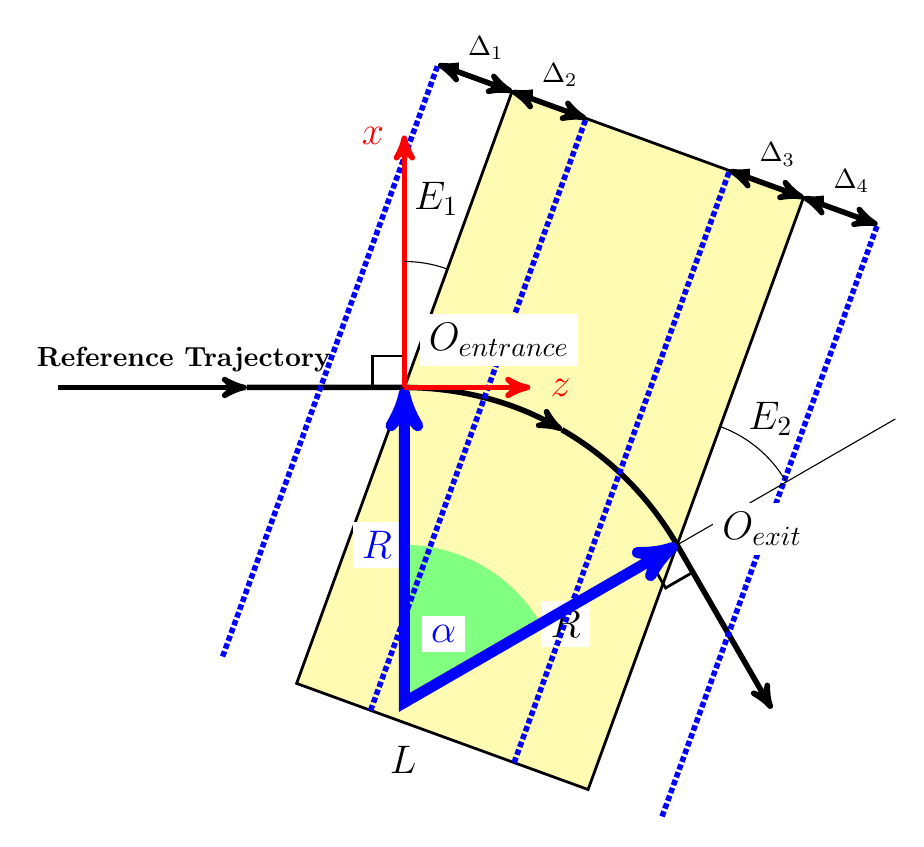
\begin{tikzpicture}[scale=4]
    \pgfmathsetmacro\Alpha{60}
    \pgfmathsetmacro\E2{40}
    \pgfmathsetmacro\sinAlpha{sin(\Alpha)}
    \pgfmathsetmacro\cosAlpha{cos(\Alpha)}
    \pgfmathsetmacro\sinAlphaHalf{sin(0.5*\Alpha)}
    \pgfmathsetmacro\cosAlphaHalf{cos(0.5*\Alpha)}
    \pgfmathsetmacro\width{2*\sinAlphaHalf*cos(10)}
    \pgfmathsetmacro\sinE2Half{sin(0.5*\E2)}
    \pgfmathsetmacro\cosE2Half{cos(0.5*\E2)}

      % First draw rectangular magnet shape.
      \begin{scope}[rotate=-20]
        \node[above=2pt] at (0.433012701892,-1.2) {\Large{\textbf{\color{black}$L$}}};
        \draw[line width=1pt,fill=yellow!30!white] (0,-1.0) rectangle (\width,1.0);
      \end{scope}

      % Now draw squares indicating 90 degree angles to bend radius at entrance and exit.
      \draw[line width=1pt] (0.0,0.0) rectangle (-0.1,0.1);
      \draw[line width=1pt,rotate around={-\Alpha:(0.0,-1.0)}]
      (0.0,-0.1) rectangle (0.1,0.0);

      % Draw reference particle path.
      \node[above=2pt] at (-0.7,0.0) {\textbf{\color{black}Reference Trajectory}};
      \draw[arrows=->,line width=2pt] (-1.1,0.0) -- (-0.5,0.0);
      \draw[arrows=->,line width=2pt] (-0.5, 0.0) -- (0.0,0.0) arc (90:60:1.0);
      \draw[arrows=->,line width=2pt] ($(0.0, -1.0) + (\sinAlphaHalf, \cosAlphaHalf)$) arc (60:30:1.0) -- +(-60:0.6);%1.1160254,-0.9330127);

      % Draw bend angle.
      \fill[green!50!white] (0.0,-1.0) -- (0.0,-0.5) arc (90:30:0.5) -- (0.0,-1.0);
      \node[fill=white] at ($(0.0,-1.0) + 0.25*(\sinAlphaHalf,\cosAlphaHalf)$) {\Large{\textbf{\color{blue}$\alpha$}}};

      \node[blue,left=1pt,fill=white] at (0.0, -0.5) {\Large{\textbf{$R$}}};
      \node[below=6pt,right=0pt,fill=white] at ($(0,-1) + 0.5*(\sinAlpha,\cosAlpha)$) {\Large{\textbf{$R$}}};
      \draw[arrows=<->,blue,line width=4pt]  (0,0) -- (0.0,-1.0) -- ($(0,-1) + (\sinAlpha, \cosAlpha)$);

      \begin{scope}[rotate=-20]
        % Draw entrance fringe field region.
        \draw[blue, densely dotted, line width=2pt] (-0.25, -1.0) -- (-0.25, 1.0);
        \draw[blue, densely dotted, line width=2pt] (0.25, -1.0) -- (0.25, 1.0);
        \draw[arrows=<->, line width=2pt] (-0.25, 1.0) -- (0.0, 1.0);
        \draw[arrows=<->, line width=2pt] (0.25, 1.0) -- (0.0, 1.0);
        \filldraw[white] (-0.125, 1.1) circle (0.1pt)
        node[fill=white] {\textbf{\color{black}$\Delta_{1}$}};
        \filldraw[white] (0.125, 1.1) circle (0.1pt)
        node[fill=white] {\textbf{\color{black}$\Delta_{2}$}};

        % Draw exit fringe field region.
        \draw[blue, densely dotted, line width=2pt] ($(\width, -1.0) - (0.25,0)$) -- ($(\width, 1.0) - (0.25,0)$);
        \draw[blue, densely dotted, line width=2pt] ($(\width, -1.0) + (0.25,0)$) -- ($(\width, 1.0) + (0.25,0)$);
        \draw[arrows=<->, line width=2pt] ($(\width, 1.0) - (0.25,0)$) -- (\width, 1.0);
        \draw[arrows=<->, line width=2pt] (\width, 1.0) -- ($(\width, 1.0) + (0.25,0)$);
        \node[fill=white] at ($(\width, 1.1) - (0.125,0)$) {\textbf{\color{black}$\Delta_{3}$}};
        \node[fill=white] at ($(\width, 1.1) + (0.125,0)$) {\textbf{\color{black}$\Delta_{4}$}};
      \end{scope}

      % Draw reference axes.
      \draw[red,arrows=->,line width=2pt] (0.0,0.0) -- (0.0,0.8) node[fill=white,left=3pt] {\Large{\textbf{$x$}}};
      \draw[red,arrows=->,line width=2pt] (0.0,0.0) -- (0.4,0.0) node[right=3pt] {\Large{\textbf{$z$}}};

      \draw (0.0, 0.4) arc (90:70:0.4);
      \node[anchor=west] at (0.0, 0.6) {\Large{$E_1$}};
      \draw ($(0,-1) + (\sinAlpha,\cosAlpha)$) -- ($(0,-1) + 1.8*(\sinAlpha,\cosAlpha)$);
      \draw ($(0,-1) + 1.4*(\sinAlpha,\cosAlpha)$) arc (30:70:0.4);
      \node at ($(1.4*\sinAlpha,-1+1.4*\cosAlpha) + (-0.05,0.2)$) {\Large{$E_2$}};

	% Label reference trajector entry and exit points.
   	\node[fill=white] at (0.3, 0.15) {\Large{$O_{entrance}$}};
	\node[fill=white, below=12pt, right=3pt] at ($(0,-1) + 1.1*(\sinAlpha,\cosAlpha)$) {\Large{\textbf{$O_{exit}$}}};
    \end{tikzpicture}
  \end{center}
  \caption{Illustration of a rectangular bend (\keyword{RBEND}, see \ssecref{RBend}) showing the entrance and exit fringe field regions. $\Delta_{1}$ is the perpendicular distance in front of the entrance edge of the magnet where the magnet fringe fields are non-negligible. $\Delta_{2}$ is the perpendicular distance behind the entrance edge of the magnet where the entrance Enge function stops being used to calculate the magnet field. The reference trajectory entrance point is indicated by $O_{entrance}$. $\Delta_{3}$ is the perpendicular distance in front of the exit edge of the magnet where the exit Enge function starts being used to calculate the magnet field. (In the region between $\Delta_{2}$ and $\Delta_{3}$ the field of the magnet is a constant value.) $\Delta_{4}$ is the perpendicular distance after the exit edge of the magnet where the magnet fringe fields are non-negligible. The reference trajectory exit point is indicated by $O_{exit}$}
  \label{fig:rbendengetype1}
\end{figure}

\begin{figure}[ht]
  \begin{center}
    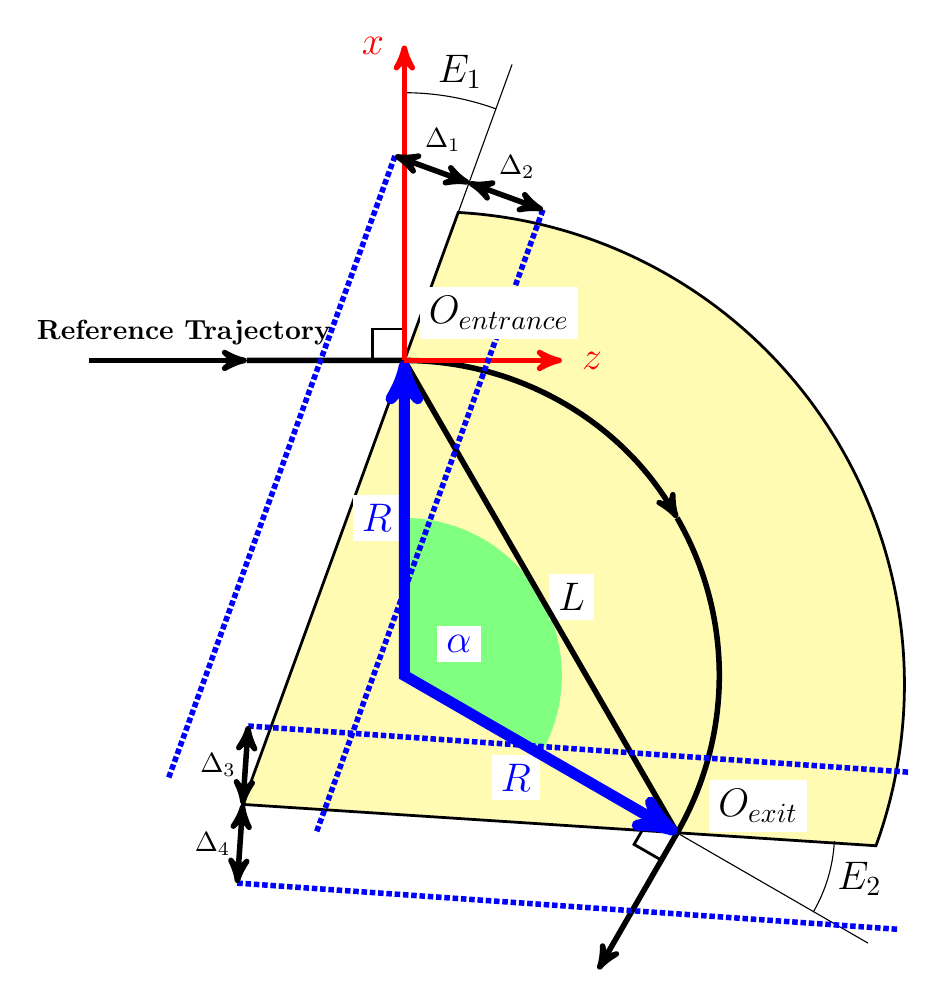
\begin{tikzpicture}[scale=4]
      % Draw magnet shape.
      \begin{scope}[rotate=-20]
        \draw[line width=1pt,fill=yellow!30!white] (0.0,-1.5)
        -- ((0.0,0.5) arc (106.82:0:1.5) -- cycle;
        \draw (0,0.5) -- (0,1);
        \draw (0,0.85) arc (90:98:0.85) node[anchor=south] {\Large{$E_1$}} arc(98:110:0.85);
      \end{scope}

      % Now draw squares indicating 90 degree angles to bend radius at entrance and exit.
      \draw[line width=1pt] (0.0,0.0) rectangle (-0.1,0.1);
      \draw[line width=1pt,xshift=0.8660254cm,yshift=-1.5cm,rotate around={60:(0.0,0.0)}]
      (-0.1,0.0) rectangle (0.0,0.1);

      % Draw reference particle path.
      \node[above=2pt] at (-0.7,0.0) {\textbf{\color{black}Reference Trajectory}};
      \draw[arrows=->,line width=2pt] (-1.,0.0) -- (-0.5,0.0);
      \draw[arrows=->,line width=2pt] (-0.5,0.0) -- (0.0,0.0) arc (90:30:1.0);
      \draw[arrows=->,line width=2pt] (0.8660254,-0.5) arc (30:-30:1.0)-- (0.6160254,-1.9330127);

      % Draw bend angle.
      \fill[green!50!white] (0.0,-1.0) -- (0.0,-0.5) arc (90:-30:0.5) -- (0.0,-1.0);
      \draw[green!50!white] (0.0,-0.8) arc (90:30:0.2)
      node[fill=white] {\Large{\textbf{\color{blue}$\alpha$}}};

      % Label chord length.
      \draw[line width=2pt] (0.0,0.0) -- (0.4330127,-0.75)
      node[fill=white,right=2pt] {\Large{\textbf{\color{black}$L$}}};
      \draw[line width=2pt] (0.4330127,-0.75) -- (0.8660254,-1.5);

      \node[blue,left=1pt,fill=white] at (0.0, -0.5) {\Large{\textbf{$R$}}};

      \node[blue,anchor=north east,fill=white] at (0.4330217,-1.25) {\Large{\textbf{$R$}}};
      \draw[arrows=<->,blue,line width=4pt] (0,0) -- (0,-1) -- (0.8660254,-1.5);
      \draw (0.8660254,-1.5) -- ($(1.7*0.8660254,-1-1.7*0.5)$);
      \draw ($(1.5*0.8660254,-1-1.5*0.5)$) arc (-30:-17:0.5) node[anchor=west] {\Large{$E_2$}} arc (-17:-3:0.5);
     % Draw reference axes.
      \draw[red,arrows=->,line width=2pt] (0.0,0.0) -- (0.0,1.0) node[left=3pt] {\Large{\textbf{$x$}}};
      \draw[red,arrows=->,line width=2pt] (0.0,0.0) -- (0.5,0.0) node[right=3pt] {\Large{\textbf{$z$}}};

      % Draw entrance fringe field region.
      \begin{scope}[rotate=-20]
        \draw[blue, densely dotted, line width=2pt] (-0.25, -1.5) -- (-0.25, 0.6);
        \draw[blue, densely dotted, line width=2pt] (0.25, -1.5) -- (0.25, 0.6);
        \draw[arrows=<->, line width=2pt] (-0.25, 0.6) -- (0.0, 0.6);
        \draw[arrows=<->, line width=2pt] (0.25, 0.6) -- (0.0, 0.6);
        \filldraw[white] (-0.125, 0.7) circle (0.1pt)
        node {\textbf{\color{black}$\Delta_{1}$}};
        \filldraw[white] (0.125, 0.7) circle (0.1pt)
        node {\textbf{\color{black}$\Delta_{2}$}};
      \end{scope}

      % Draw exit fringe field region.
      \begin{scope}[rotate around={-94:(-0.513,-1.410)}]
        \draw[blue, densely dotted, line width=2pt] (-0.763,-1.410) -- (-0.763,0.690);
        \draw[blue, densely dotted, line width=2pt] (-0.263,-1.410) -- (-0.263,0.690);
        \draw[arrows=<->,line width=2pt] (-0.763,-1.410) -- (-0.513,0.-1.410);
        \draw[arrows=<->,line width=2pt] (-0.263,-1.410) -- (-0.513,-1.410);
        \node[anchor=east] at (-0.638,-1.410) {\textbf{$\Delta_{3}$}};
        \node[anchor=east] at (-0.388,-1.410) {\textbf{$\Delta_{4}$}};
      \end{scope}

	% Label reference trajector entry and exit points.
   	\node[fill=white] at (0.3, 0.15) {\Large{$O_{entrance}$}};
   	\node[anchor=north east,fill=white] at (1.28,-1.33) {\Large{\textbf{$O_{exit}$}}};

    \end{tikzpicture}
  \end{center}
  \caption{Illustration of a sector bend (\keyword{SBEND}, see \ssecref{SBend}) showing the entrance and exit fringe field regions. $\Delta_{1}$ is the perpendicular distance in front of the entrance edge of the magnet where the magnet fringe fields are non-negligible. $\Delta_{2}$ is the perpendicular distance behind the entrance edge of the magnet where the entrance Enge function stops being used to calculate the magnet field. The reference trajectory entrance point is indicated by $O_{entrance}$. $\Delta_{3}$ is the perpendicular distance in front of the exit edge of the magnet where the exit Enge function starts being used to calculate the magnet field. (In the region between $\Delta_{2}$ and $\Delta_{3}$ the field of the magnet is a constant value.) $\Delta_{4}$ is the perpendicular distance after the exit edge of the magnet where the magnet fringe fields are non-negligible. The reference trajectory exit point is indicated by $O_{exit}$.}
  \label{fig:sbendengetype1}
\end{figure}

%\clearpage

\subsection{1DProfile1 Type 1 for Bend Magnet}
\label{ssec:1DProfile1Type1}
A \texttt{1DProfile1 Type 1} field map is the same \texttt{1DProfile1} field map found in versions of \opal previous to
\opal \opalversion{1.2.0} . \figref{rbendengetype1,sbendengetype1} illustrate the fringe field
regions for an \keyword{RBEND} and an \keyword{SBEND} element. Referring to the general field map file shown in
\tabref{1DProfile1}, the values on lines 2 and 3 are given by:

\begin{align*}
  Entrance\,Parameter\,1 &= Entrance\,Parameter\,2 - \Delta_{1} \\
  Entrance\,Parameter\,3 &= Entrance\,Parameter\,2 + \Delta_{2} \\
  Exit\,Parameter\,2 &= L - Entrance\,Parameter\,2 \\
  Exit\,Parameter\,1 &= Exit\,Parameter\,2 - \Delta_{3} \\
  Exit\,Parameter\,3 &= Exit\,Parameter\,2 + \Delta_{4}
\end{align*}
The value of $Entrance\,Parameter\,2$ can be any value. \opal only cares about the relative differences between
parameters. Also note that, internally, the origins of the entrance and exit Enge functions correspond to the
reference trajectory entrance and exit points \seefig{rbendengetype1,sbendengetype1}.

Internally, \opal reads in a \texttt{1DProfile Type 1} map and uses the provided parameters to calculate the values of:

\begin{align*}
L &= Exit\,Parameter\,2 - Entrance\,Parameter\,2 \\
\Delta_{1} &= Entrance\,Parameter\,2 - Entrance\,Parameter\,1 \\
\Delta_{2} &= Entrance\,Parameter\,3 - Entrance\,Parameter\,2 \\
\Delta_{3} &= Exit\,Parameter\,2 - Exit\,Parameter\,1 \\
\Delta_{4} &= Exit\,Parameter\,3 - Exit\,Parameter\,2
\end{align*}
These values, combined with the entrance fringe field Enge coefficients $c_0$ through $c_{N_{Enge_Entrance}}$ and exit fringe field Enge coefficients $c_0$ through $c_{N_{Enge_Exit}}$, allow \opal to find field values anywhere within the magnet. (Again, note that a \texttt{1DProfile Type 1} map always places the entrance Enge function origin at the entrance point of the reference trajectory and the exit Enge function origin at the exit point of the reference trajectory.)

\figref{1DProfile1Type1} shows an example of a \texttt{1DProfile1 Type 1} field map file.

\begin{figure}[ht]
  \begin{fmpage}
\begin{verbatim}
1DProfile1 6 7 3.0
-6.0 -2.0 2.0  1000
24.0 28.0 32.0 0
  0.00000e+00
  4.36222e-06
  8.83270e-06
  + 9 lines
  1.32490e-05
  1.73710e-05
  2.18598e-05
\end{verbatim}
  \end{fmpage}
  \caption[Example of a 1DProfile1 Type 1 field map]{A 1D field map describing the fringe field of an element using
    7 Enge coefficients for the entrance fringe field and 8 Enge coefficients for the exit fringe field (polynomial
    order 6 and 7 respectively). The element has a gap height of \SI{3.0}{\centi\meter}, and a length of \SI{30.0}{\centi\meter}. The entrance
    fringe field is non-negligible from \SI{4.0}{\centi\meter} in front of the magnet's entrance edge and reaches the core strength
    at \SI{4.0}{\centi\meter} behind the entrance edge of the magnet. (The entrance edge position is given by the element's
    \keyword{ELEMEDGE} attribute.) The exit fringe field region begins \SI{4.0}{\centi\meter} in front of the exit edge of the magnet and is non-negligible \SI{4.0}{\centi\meter} after the exit edge of the magnet. The value 1000 at the end of line 2 and 0 at the end of line 3 do not have any meaning.}
  \label{fig:1DProfile1Type1}
\end{figure}

%\clearpage

\subsection{1DProfile1 Type 2 for Bend Magnet}
\label{ssec:1DProfile1Type2}
The \texttt{1DProfile1 Type 2} field map file format was introduce in \opal \opalversion{1.2.0} to allow for more flexibility
when defining the Enge functions for the entrance and exit fringe fields. Specifically, a \texttt{1DProfile1 Type 2} map
does not contain any information about the length of the magnet. Instead, that value is set using the element's
\keyword{L} attribute. In turn, this allows us the freedom to make slight changes to how the parameters on lines 2
and 3 of the field map file shown in \tabref{1DProfile1} are defined. Now

\begin{align*}
  Entrance\,Parameter\,2 &= \perp \text{distance of entrance Enge function origin from magnet entrance edge} \\
  Exit\,Parameter\,2 &= \perp \text{distance of exit Enge function origin from magnet exit edge}
\end{align*}
The other parameters are defined the same as before:

\begin{align*}
  Entrance\,Parameter\,1 &= Entrance\,Parameter\,2 - \Delta_{1} \\
  Entrance\,Parameter\,3 &= Entrance\,Parameter\,2 + \Delta_{2} \\
  Exit\,Parameter\,1 &= Exit\,Parameter\,2 - \Delta_{3} \\
  Exit\,Parameter\,3 &= Exit\,Parameter\,2 + \Delta_{4}
\end{align*}

As before, internally, \opal reads in a \texttt{1DProfile Type 2} map and uses the provided parameters to calculate the values of:
\begin{align*}
\Delta_{1} &= Entrance\,Parameter\,2 - Entrance\,Parameter\,1 \\
\Delta_{2} &= Entrance\,Parameter\,3 - Entrance\,Parameter\,2 \\
\Delta_{3} &= Exit\,Parameter\,2 - Exit\,Parameter\,1 \\
\Delta_{4} &= Exit\,Parameter\,3 - Exit\,Parameter\,2
\end{align*}
These values, combined with the length of the magnet, \keyword{L} ( set by the element attribute) and the entrance fringe field Enge coefficients $c_0$ through $c_{N_{Enge_Entrance}}$ and exit fringe field Enge coefficients $c_0$ through $c_{N_{Enge_Exit}}$, allow \opal to find field values anywhere within the magnet.

The \texttt{1DProfile1 Type 2} field map file format has two main advantages:

\begin{enumerate}
\item The Enge function origins can be adjusted to more accurately model a magnet's fringe fields as they are no longer fixed to the entrance and exit points of the reference trajectory.
\item Two magnets with the same fringe fields, but different lengths, can be modeled with a single
  \texttt{1DProfile Type 2} field map file rather than two separate files.
\end{enumerate}
\figref{1DProfile1Type2} shows an example of a \texttt{1DProfile1 Type 2} field map file.

\begin{figure}[h]
  \begin{fmpage}
\begin{verbatim}
1DProfile1 6 7 3.0
-6.0 -2.0 2.0 0
-2.0  2.0 6.0 0
  0.00000e+00
  4.36222e-06
  8.83270e-06
  + 9 lines
  1.32490e-05
  1.73710e-05
  2.18598e-05
\end{verbatim}
\end{fmpage}
\caption[Example of a 1DProfile1 Type 2 field map]{A 1D field map describing the fringe field of an element using 7 Enge coefficients for the entrance fringe field and 8 Enge coefficients for the exit fringe field (polynomial order 6 and 7 respectively). The element has a gap height of \SI{3.0}{\centi\meter}. The entrance fringe field is non-negligible from \SI{4.0}{\centi\meter} in front of the magnet's entrance edge and reaches the core strength at \SI{4.0}{\centi\meter} behind the entrance edge of the magnet. The exit fringe field region begins \SI{4.0}{\centi\meter} in front of the exit edge of the magnet and is non-negligible \SI{4.0}{\centi\meter} after the exit edge of the magnet. The value 0 at the end of line 2 and 0 at the end of line 3 do not have any meaning. The entrance Enge function origin is \SI{2.0}{\centi\meter} in front (upstream) of the magnet's entrance edge. The exit Enge function origin is \SI{2.0}{\centi\meter} behind (downstream of) the exit edge of the magnet.}
\label{fig:1DProfile1Type2}
\end{figure}

%\clearpage


\section{2DElectroStatic}
\label{sec:2DElectroStatic}
\index{2DElectroStatic}
\index{Field Map!2DElectroStatic}
\begin{figure}[h]
  \begin{fmpage}
\begin{verbatim}
2DElectroStatic XZ
-3.0 51.0 4999
0.0 2.0 199
  0.00000e+00  0.00000e+00
  4.36222e-06  0.00000e+00
  8.83270e-06  0.00000e+00
  + 999994 lines
  1.32490e-05  0.00000e+00
  1.73710e-05  0.00000e+00
  2.18598e-05  0.00000e+00
\end{verbatim}
  \end{fmpage}
  \caption[Example of a 2DElectroStatic field map]{A 2D field map describing an electrostatic field using 5000 grid points
    in the longitudinal direction times 200 grid points in the radial direction. The field between the grid points is calculated
    using bi-linear interpolation. The field is non-negligible from \SI{-3.0}{\centi\meter} to \SI{51.0}{\centi\meter} relative to \keyword{ELEMEDGE} and the 200
    grid points in the radial direction span the distance from \SI{0.0}{\centi\meter} to \SI{2.0}{\centi\meter}. The field values are ordered in XZ
    orientation, so the index in the longitudinal direction changes fastest and therefore $E_z$ values are stored in the first
    column and $E_r$ values in the second \seesec{fieldorientation}. \opalt normalizes the field so that $max(|E_{z, \text{ on axis}}|) = \SI{1}{\mega\volt\per\meter}$.}
  \label{fig:2DElectroStatic}
\end{figure}

\begin{table}[ht!]
    \caption{Layout of a \texttt{2DElectroStatic} field map file.}
    \label{tab:2DElectroStatic}
    \begin{center}
    \begin{tabular}{lll}
      \hline
      2DElectroStatic & Orientation (XZ or ZX) & \\
      $z_{start}$ (or $r_{start}$) (in cm) & $z_{end}$ (or $r_{end}$) (in cm) & $N_{z}$ (or $N_{r}$) \\
      $r_{start}$ (or $z_{start}$) (in cm) & $r_{end}$ (or $z_{end}$) (in cm) & $N_{r}$ (or $N_{z}$) \\
      $E_{z,\,1}$ (or $E_{r,\,1}$) (MV/m) & $E_{r,\,1}$ (or $E_{z,\,1}$) (MV/m)& \\
      $E_{z,\,2}$ (or $E_{r,\,2}$) (MV/m) & $E_{r,\,2}$ (or $E_{z,\,2}$) (MV/m)& \\
      . & & \\
      . & & \\
      . & & \\
      $E_{z,\,N}$ (or $E_{r,\,N}$) (MV/m) & $E_{r,\,N}$ (or $E_{z,\,N}$) (MV/m)& \\
      \hline
    \end{tabular}
    \end{center}
\end{table}

A \texttt{2DElectroStatic} field map has the general form shown in \tabref{2DElectroStatic}. The first three lines form
the file header and tell \opalt how the field map data is being presented:

\begin{description}
\item[Line 1] This tells \opalt what type of field file it is (\texttt{2DElectroStatic}) and the field orientation
  \seesec{fieldorientation}.
\item[Line 2] This gives the extent of the field map and how many grid spacings there are in the fastest changing
  index direction \seesec{fieldorientation}.
\item[Line 3] This gives the extent of the field map and how many grid spacings there are in the slowest changing
  index direction (see \secref{fieldorientation}.
\end{description}

The lines following the header give the 2D field map grid values from $1$ to $N = (N_{z} + 1) \times (N_{r} + 1)$.
The order of these depend on the field orientation \seesec{fieldorientation} and can be one of two formats:

\begin{description}
\item[If Orientation = XZ:] $E_{z}$ (MV/m) $E_{r}$ (MV/m)
\item[If Orientation = ZX:] $E_{r}$ (MV/m) $E_{z}$ (MV/m)
\end{description}

\figref{2DElectroStatic} gives an example of a \texttt{2DElectroStatic} field file.

%\clearpage

\section{2DMagnetoStatic}
\label{sec:2DMagnetoStatic}
\index{2DMagnetoStatic}
\index{Field Map!2DMagnetoStatic}
\begin{figure}[h]
  \begin{fmpage}
\begin{verbatim}
2DMagnetoStatic ZX
0.0 2.0 199
-3.0 51.0 4999
  0.00000e+00  0.00000e+00
  0.00000e+00  4.36222e-06
  0.00000e+00  8.83270e-06
  + 999994 lines
  0.00000e+00  1.32490e-05
  0.00000e+00  1.73710e-05
  0.00000e+00  2.18598e-05
\end{verbatim}
  \end{fmpage}
  \caption[Example of a 2DMagnetoStatic field map]{A 2D field map describing a magnetostatic field using 5000 grid points
    in the longitudinal direction times 200 grid points in the radial direction. The field between the grid points is calculated
    using bi-linear interpolation. The field is non-negligible from \SI{-3.0}{\centi\meter} to \SI{51.0}{\centi\meter} relative to \keyword{ELEMEDGE} and the 200 grid
    points in the radial direction span the distance from \SI{0.0}{\centi\meter} to \SI{2.0}{\centi\meter}. The field values are ordered in the ZX
    orientation, so the index in the radial direction changes fastest and therefore $B_r$ values are stored in the first column
    and $B_z$ values in the second \seesec{fieldorientation}. \opalt normalizes the field so that $max(|B_{z,\text{ on axis}}|) = \SI{1}{\tesla}$.}
  \label{fig:2DMagnetoStatic}
\end{figure}

\begin{table}[ht!]
    \caption{Layout of a \texttt{2DMagnetoStatic} field map file.}
    \label{tab:2DMagnetoStatic}
    \begin{center}
    \begin{tabular}{lll}
      \hline
      2DMagnetoStatic & Orientation (XZ or ZX) & \\
      $z_{start}$ (or $r_{start}$) (in cm) & $z_{end}$ (or $r_{end}$) (in cm) & $N_{z}$ (or $N_{r}$) \\
      $r_{start}$ (or $z_{start}$) (in cm) & $r_{end}$ (or $z_{end}$) (in cm) & $N_{r}$ (or $N_{z}$) \\
      $B_{z,\,1}$ (or $B_{r,\,1}$) (T) & $B_{r,\,1}$ (or $B_{z,\,1}$) (T)& \\
      $B_{z,\,2}$ (or $B_{r,\,2}$) (T) & $B_{r,\,2}$ (or $B_{z,\,2}$) (T)& \\
      . & & \\
      . & & \\
      . & & \\
      $B_{z,\,N}$ (or $B_{r,\,N}$) (T) & $B_{r,\,N}$ (or $B_{z,\,N}$) (T)& \\
      \hline
    \end{tabular}
    \end{center}
\end{table}

A \texttt{2MagnetoStatic} field map has the general form shown in \tabref{2DMagnetoStatic}. The first three lines form
the file header and tell \opalt how the field map data is being presented:

\begin{description}
\item[Line 1] This tells \opalt what type of field file it is (\texttt{2DMagnetoStatic}) and the field orientation
  \seesec{fieldorientation}.
\item[Line 2] This gives the extent of the field map and how many grid spacings there are in the fastest changing
  index direction \seesec{fieldorientation}.
\item[Line 3] This gives the extent of the field map and how many grid spacings there are in the slowest changing
  index direction (see \secref{fieldorientation}.
\end{description}

The lines following the header give the 2D field map grid values from $1$ to $N = (N_{z} + 1) \times (N_{r} + 1)$.
The order of these depend on the field orientation \seesec{fieldorientation} and can be one of two formats:

\begin{description}
\item[If Orientation = XZ:] $B_{z}$ (T) $B_{r}$ (T)
\item[If Orientation = ZX:] $B_{r}$ (T)  $B_{z}$ (T)
\end{description}

\figref{2DMagnetoStatic} gives an example of a \texttt{2DMagnetoStatic} field file.

%\clearpage

\section{2DDynamic}
\label{sec:2DDynamic}
\index{2DDynamic}
\index{Field Map!2DDynamic}
\begin{figure}[h]
  \begin{fmpage}
\begin{verbatim}
2DDynamic XZ
-3.0 51.0 4121
1498.953425154
0.0 1.0 75
  0.00000e+00  0.00000e+00  0.00000e+00  0.00000e+00
  4.36222e-06  0.00000e+00  0.00000e+00  4.36222e-06
  8.83270e-06  0.00000e+00  0.00000e+00  8.83270e-06
  + 313266 lines
  1.32490e-05  0.00000e+00  0.00000e+00  1.32490e-05
  1.73710e-05  0.00000e+00  0.00000e+00  1.73710e-05
  2.18598e-05  0.00000e+00  0.00000e+00  2.18598e-05
\end{verbatim}
  \end{fmpage}
  \caption[Example of a 2DDynamic field map]{A 2D field map describing a dynamic field oscillating with a frequency of
    \SI{1498.953425154}{\mega\hertz}. The field map provides 4122 grid points in the longitudinal direction times 76 grid points in
    radial direction. The field between the grid points is calculated with a bi-linear interpolation. The field is
    non-negligible between \SI{-3.0}{\centi\meter} and \SI{51.0}{\centi\meter} relative to \keyword{ELEMEDGE} and the 76 grid points in radial direction
    span the distance from \SI{0.0}{\centi\meter} to \SI{1.0}{\centi\meter}. The field values are ordered in the XZ orientation, so the index in the
    longitudinal direction changes fastest and therefore $E_z$ values are stored in the first column and $E_r$ values
    in the second. The third column contains the electric field magnitude, $|E|$, and is not used (but must still be included).
    The fourth column is $H_{\phi}$ in A/m. The third and fourth columns are always the same and do not depend on the field
    orientation \seesec{fieldorientation}. \opalt normalizes the field so that $max(|E_{z,\text{ on axis}}|) = \SI{1}{\mega\volt\per\meter}$.}
  \label{fig:2DDynamic}
\end{figure}

\begin{table}[ht!]
    \caption{Layout of a \texttt{2DDynamic} field map file.}
    \label{tab:2DDynamic}
    \begin{center}
    \begin{tabular}{llll}
      \hline
      2DDynamic & Orientation (XZ or ZX) & & \\
      $z_{start}$ (or $r_{start}$) (in cm) & $z_{end}$ (or $r_{end}$) (in cm) & $N_{z}$ (or $N_{r}$)& \\
      $Frequency$ (in MHz) & & & \\
      $r_{start}$ (or $z_{start}$) (in cm) & $r_{end}$ (or $z_{end}$) (in cm) & $N_{r}$ (or $N_{z}$)& \\
      $E_{z,\,1}$ (or $E_{r,\,1}$) (MV/m)) & $E_{r,\,1}$ (or $E_{z,\,1}$) (MV/m) & $|E_1|$ (MV/m) & $H_{\phi,\,1}$ (A/m) \\
      $E_{z,\,2}$ (or $E_{r,\,2}$) (MV/m)) & $E_{r,\,2}$ (or $E_{z,\,2}$) (MV/m) & $|E_2|$ (MV/m) & $H_{\phi,\,2}$ (A/m) \\
      . & & \\
      . & & \\
      . & & \\
      $E_{z,\,N}$ (or $E_{r,\,N}$) (MV/m)) & $E_{r,\,N}$ (or $E_{z,\,N}$) (MV/m) & $|E_N|$ (MV/m) & $H_{\phi,\,N}$ (A/m) \\
      \hline
    \end{tabular}
    \end{center}
\end{table}

A \texttt{2DDynamic} field map has the general form shown in \tabref{2DDynamic}. The first four lines form
the file header and tell \opalt how the field map data is being presented:

\begin{description}
\item[Line 1] This tells \opalt what type of field file it is (\texttt{2DDynamic}) and the field orientation
  \seesec{fieldorientation}.
\item[Line 2] This gives the extent of the field map and how many grid spacings there are in the fastest changing
  index direction \seesec{fieldorientation}.
\item[Line 3] Field frequency.
\item[Line 4] This gives the extent of the field map and how many grid spacings there are in the slowest changing
  index direction \seesec{fieldorientation}.
\end{description}

The lines following the header give the 2D field map grid values from $1$ to $N= (N_{z} + 1) \times (N_{r} + 1)$. The
order of these depend on the field orientation \seesec{fieldorientation} and can be one of two formats:
\begin{description}
\item[If Orientation = XZ:] $E_{z}$ (MV/m) $E_{r}$ (MV/m) $|E|$ (MV/m) $H_{\phi}$ (A/m)
\item[If Orientation = ZX:] $E_{r}$ (MV/m) $E_{z}$ (MV/m) $|E|$ (MV/m) $H_{\phi}$ (A/m)
\end{description}
The third item (the field magnitude) on each data line is not used by \opalt, but must be there.

\figref{2DDynamic} gives an example of a \texttt{2DDynamic} field file.
%\clearpage
\section{3DMagnetoStatic}
\label{sec:3DMagnetoStatic}
\index{3DMagnetoStatic}
\index{Field Map!3DMagnetoStatic}
\begin{figure}[h]
  \begin{fmpage}
\begin{verbatim}
3DMagnetoStatic
-1.5 1.5 227
-1.0 1.0 151
-3.0 51.0 4121
0.00e+00 0.00e+00 0.00e+00
0.00e+00 4.36e-06 0.00e+00
0.00e+00 8.83e-06 0.00e+00
+ 142'852'026 lines
0.00e+00 1.32e-05 0.00e+00
0.00e+00 1.73e-05 0.00e+00
0.00e+00 2.18e-05 0.00e+00
\end{verbatim}
  \end{fmpage}
  \caption[Example of a 3DMagnetoStatic field map]{A 3D field map describing a magnetostatic field.
    The field map provides 4122 grid points in z-direction times 228 grid points in x-direction and 152 grid points in y-direction.
    The field between the grid points is calculated with a tri-linear interpolation. The field is non-negligible between \SI{-3.0}{\centi\meter}
    to \SI{51.0}{\centi\meter} relative to \keyword{ELEMEDGE}, the 228 grid points in x-direction range from \SI{-1.5}{\centi\meter} to \SI{1.5}{\centi\meter} and the 152 grid
    points in y-direction range from \SI{-1.0}{\centi\meter} to \SI{1.0}{\centi\meter} relative to the design path. The field values are ordered such that the index in z-direction changes fastest, then the index in y-direction while the index in x-direction changes
    slowest. The columns correspond to $B_x$, $B_y$ and $B_z$.}
  \label{fig:3DMagnetoStatic}
\end{figure}

\begin{table}[ht!]
    \caption{Layout of a \texttt{3DMagnetoStatic} field map file.}
    \label{tab:3DMagnetoStatic}
    \begin{center}
    \begin{tabular}{llllll}
      \hline
      3DMagnetoStatic     &                   &                   \\
      $x_{start}$ (in cm) & $x_{end}$ (in cm) & $N_{x}$           \\
      $y_{start}$ (in cm) & $y_{end}$ (in cm) & $N_{y}$           \\
      $z_{start}$ (in cm) & $z_{end}$ (in cm) & $N_{z}$           \\
      $B_{x,\,1}$ (A/m)   & $B_{y,\,1}$ (A/m) & $B_{z,\,1}$ (A/m) \\
      $B_{x,\,2}$ (A/m)   & $B_{y,\,2}$ (A/m) & $B_{z,\,2}$ (A/m) \\
      .                   &                   &                   \\
      .                   &                   &                   \\
      .                   &                   &                   \\
      $B_{x,\,N}$ (A/m)   & $B_{y,\,N}$ (A/m) & $B_{z,\,N}$ (A/m) \\
      \hline
    \end{tabular}
    \end{center}
\end{table}

A \texttt{3DMagnetoStatic} field map has the general form shown in \tabref{3DMagnetoStatic}. The first five lines form
the file header and tell \opalt how the field map data is being presented:

\begin{description}
\item[Line 1] This tells \opalt what type of field file it is (\texttt{3DMagnetoStatic}).
\item[Line 3] This gives the extent of the field map and how many grid spacings there are in the slowest changing
  index direction.
\item[Line 4] This gives the extent of the field map and how many grid spacings there are in the next fastest changing
  index direction.
\item[Line 5] This gives the extent of the field map and how many grid spacings there are in the fastest changing
  index direction.
\end{description}

The lines following the header give the 3D field map grid values from $1$ to $N= (N_{z} + 1) \times (N_{y} + 1) \times (N_{x} + 1)$.
\figref{3DMagnetoStatic} gives an example of a \texttt{3DMagnetoStatic} field file.

\newpage
\section{3DMagnetoStatic\_Extended}
\label{sec:3DMagnetoStatic_Extended}
\index{3DMagnetoStatic\_Extended}
\index{Field Map!3DMagnetoStatic\_Extended}
\begin{figure}[h]
  \begin{fmpage}
\begin{verbatim}
3DMagnetoStatic_Extended
-9.9254 9.9254 133
-2.0 1.0 15
-22.425 47.425 465
 -8.10970000e-05
 -8.38540000e-05
 -8.64960000e-05
+ 62'438 lines
 -8.64960000e-05
 -8.38540000e-05
 -8.10970000e-05
\end{verbatim}
  \end{fmpage}
  \caption[Example of a 3DMagnetoStatic\_Extended field map]{A 3D field map describing a magnetostatic field on the mid-plane. The field map provides 466 grid points in z-direction times 134 grid points in x-direction. The field is non-negligible between \SI{-22.425}{\centi\meter} to \SI{47.425}{\centi\meter} relative to \keyword{ELEMEDGE}, the 134 grid points in x-direction range from \SI{-9.9254}{\centi\meter} to \SI{9.9254}{\centi\meter}. The field should be integrated using Maxwell's equations from the mid-plane to \SI{2.0}{\centi\meter} using 16 grid points. The mid-plane is regarded as a perfect magnetic conductor (PMC) i.e. the magnetic field on the mid-plane has no tangential component. This leads to a symmetry where the perpendicular component is mirrored whereas the tangential component is anti-parallel. Instead of integrating the field from the mid-plane to \SI{-2.0}{\centi\meter} and \SI{1.0}{\centi\meter} we only integrate it to \SI{+2.0}{\centi\meter} and store only the upper half of the field map. For positions $R(x,\;-y,\;z)$ with $y > 0.0$ the correct field can then be derived from the $R(x,\;y,\;z)$.}
  \label{fig:3DMagnetoStatic_Extended}
\end{figure}

\begin{table}[ht!]
    \caption{Layout of a \texttt{3DMagnetoStatic\_Extended} field map file.}
    \label{tab:3DMagnetoStatic_Extended}
    \begin{center}
    \begin{tabular}{lll}
      \hline
      \multicolumn{2}{l}{3DMagnetoStatic\_Extended}  &           \\
      $x_{start}$ (in cm)       & $x_{end}$ (in cm)  & $N_{x}$   \\
      $y_{start}$ (in cm)       & $y_{end}$ (in cm)  & $N_{y}$   \\
      $z_{start}$ (in cm)       & $z_{end}$ (in cm)  & $N_{z}$   \\
      $B_{y,\,1}$ (T)           &                    &           \\
      $B_{y,\,2}$ (T)           &                    &           \\
      .                         &                    &           \\
      .                         &                    &           \\
      .                         &                    &           \\
      $B_{y,\,N}$ (T)           &                    &           \\
      \hline
    \end{tabular}
    \end{center}
\end{table}

A \texttt{3DMagnetoStatic\_Extended} field map has the general form shown in \tabref{3DMagnetoStatic_Extended}. The first four lines form the file header and tell \opalt how the field map data is being presented:

\begin{description}
\item[Line 1] This tells \opalt what type of field file it is (\texttt{3DMagnetoStatic\_Extended}).
\item[Line 2] This gives the extent of the field map and how many grid spacings there are in the slowest changing direction.
\item[Line 3] This gives the extent of the field map and how many grid spacings there are in the next fastest changing direction.
\item[Line 4] This gives the extent of the field map and how many grid spacings there are in the fastest changing direction.
\end{description}

The lines following the header give the 3D field map grid values from $1$ to $N= (N_{z} + 1) \times (N_{x} + 1)$.
The order of these depend on the field orientation \seesec{fieldorientation} and can currently only be the
format shown in \tabref{3DMagnetoStatic_Extended}.

\figref{3DMagnetoStatic_Extended} gives an example of a \texttt{3DMagnetoStatic\_Extended} field file.

%\clearpage
\section{3DDynamic}
\label{sec:3DDynamic}
\index{3DDynamic}
\index{Field Map!3DDynamic}
\begin{figure}[h]
  \begin{fmpage}
\begin{verbatim}
3DDynamic
1498.953425154
-1.5 1.5 227
-1.0 1.0 151
-3.0 51.0 4121
0.00e+00 0.00e+00 0.00e+00 0.00e+00 0.00e+00 0.00e+00
4.36e-06 0.00e+00 4.36e-06 0.00e+00 4.36e-06 0.00e+00
8.83e-06 0.00e+00 8.83e-06 0.00e+00 8.83e-06 0.00e+00
+ 142'852'026 lines
1.32e-05 0.00e+00 1.32e-05 0.00e+00 1.32e-05 0.00e+00
1.73e-05 0.00e+00 1.73e-05 0.00e+00 1.73e-05 0.00e+00
2.18e-05 0.00e+00 2.18e-05 0.00e+00 2.18e-05 0.00e+00
\end{verbatim}
  \end{fmpage}
  \caption[Example of a 3DDynamic field map]{A 3D field map describing a dynamic field oscillating with \SI{1.498953425154}{\giga\hertz}.
    The field map provides 4122 grid points in z-direction times 228 grid points in x-direction and 152 grid points in y-direction.
    The field between the grid points is calculated with a tri-linear interpolation. The field is non-negligible between \SI{-3.0}{\centi\meter}
    to \SI{51.0}{\centi\meter} relative to \keyword{ELEMEDGE}, the 228 grid points in x-direction range from \SI{-1.5}{\centi\meter} to \SI{1.5}{\centi\meter} and the 152 grid
    points in y-direction range from \SI{-1.0}{\centi\meter} to \SI{1.0}{\centi\meter} relative to the design path. The field values are ordered such that the index in z-direction changes fastest, then the index in y-direction while the index in x-direction changes
    slowest. The columns correspond to $E_x$, $E_y$, $E_z$, $H_x$, $H_y$ and $H_z$.}
  \label{fig:3DDynamic}
\end{figure}

\begin{table}[ht!]
    \caption{Layout of a \texttt{3DDynamic} field map file.}
    \label{tab:3DDynamic}
    \begin{center}
    \begin{tabular}{llllll}
      \hline
      3DDynamic            &                    &                    &                   &                   &                   \\
      $Frequency$ (in MHz) &                    &                    &                   &                   &                   \\
      $x_{start}$ (in cm)  & $x_{end}$ (in cm)  & $N_{x}$            &                   &                   &                   \\
      $y_{start}$ (in cm)  & $y_{end}$ (in cm)  & $N_{y}$            &                   &                   &                   \\
      $z_{start}$ (in cm)  & $z_{end}$ (in cm)  & $N_{z}$            &                   &                   &                   \\
      $E_{x,\,1}$ (MV/m))  & $E_{y,\,1}$ (MV/m) & $E_{z,\,1}$ (MV/m) & $H_{x,\,1}$ (A/m) & $H_{y,\,1}$ (A/m) & $H_{z,\,1}$ (A/m) \\
      $E_{x,\,2}$ (MV/m))  & $E_{y,\,2}$ (MV/m) & $E_{z,\,2}$ (MV/m) & $H_{x,\,2}$ (A/m) & $H_{y,\,2}$ (A/m) & $H_{z,\,2}$ (A/m) \\
      .                    &                    &                    &                   &                   &                   \\
      .                    &                    &                    &                   &                   &                   \\
      .                    &                    &                    &                   &                   &                   \\
      $E_{x,\,N}$ (MV/m))  & $E_{y,\,N}$ (MV/m) & $E_{z,\,N}$ (MV/m) & $H_{x,\,N}$ (A/m) & $H_{y,\,N}$ (A/m) & $H_{z,\,N}$ (A/m) \\
      \hline
    \end{tabular}
    \end{center}
\end{table}

A \texttt{3DDynamic} field map has the general form shown in \tabref{3DDynamic}. The first five lines form
the file header and tell \opalt how the field map data is being presented:

\begin{description}
\item[Line 1] This tells \opalt what type of field file it is (\texttt{3DDynamic}).
\item[Line 2] Field frequency.
\item[Line 3] This gives the extent of the field map and how many grid spacings there are in the slowest changing
  index direction.
\item[Line 4] This gives the extent of the field map and how many grid spacings there are in the next fastest changing
  index direction.
\item[Line 5] This gives the extent of the field map and how many grid spacings there are in the fastest changing
  index direction.
\end{description}

The lines following the header give the 3D field map grid values from $1$ to $N= (N_{z} + 1) \times (N_{y} + 1) \times (N_{x} + 1)$.
\figref{3DDynamic} gives an example of a \texttt{3DDynamic} field file.

%----------- Footer control ------------------
\ifthenelse{\boolean{FullOPALManual}}
{
  %do nothing
}
% else (for individual document creation)
{
\appendix
\printbibliography
\end{document}
}
%---------------------------------------------